\documentclass[11pt]{article}
\renewcommand{\baselinestretch}{1.0}

\usepackage{amsfonts}
\usepackage{hyperref}
\usepackage{color}
\usepackage{graphicx}
\usepackage{fullpage}
\usepackage{booktabs}
\usepackage{pdfpages}
\usepackage{amsmath}
\usepackage{amssymb}
\pagestyle{empty}
\renewcommand{\baselinestretch}{1.0}
\newcommand{\ffrac}[2]{\ensuremath{\frac{\displaystyle #1}{\displaystyle #2}}}

\title{Statistics Project 1 : \\ Statistics - Math 2606}
\author{Kevin Chen, William Gantt, Nick Barnes}
\date{}
\begin{document}
\maketitle
\section{Experiment}
The assignment was to estimate the height of Searles. Although it would have been ideal to estimate the height to the top of the spire, we did not do this. Instead, we measured to the point at the top of the front facade above the door.

For the purposes of the explanation of the experiment, let the $x$-axis be the imaginary line passing through the door, parallel to the walkway that passes in front of the building, and let the $y$-axis be the line passing through the door, perpendicular to the walkway. For all measurements, we maintained a constant distance from the $x$-axis. We chose this value to be the distance from the door to a point directly in front of it, at the far edge of the walkway, where the pavement meets the grass. Call this value $a$. To vary the distance from the door to the mirror, we marked out 10 positions at 2m-intervals along the line defined by $a$ that is parallel to the $x$-axis. Call that distance to the point directly in front of the door $b$. Then our direct distance to the base of the building directly below the top of the front facade above the door is $\sqrt{a^2+b^2}$. This is a simple application of the Pythagorean theorem as our distance from the point directly in front of the door, and our distance from the point on the line parallel to the x-axis are perpendicular. 

The reader may consider that the error obtained in measuring the distance from the point directly in front of the door, and the error in measuring distance from the mirror to that point do NOT add up linearly. That is, call them $\epsilon_1$ and $\epsilon_2$, and the distance from the point perpendicular to the building $a$, the distance from the point perpendicu
\section{Results}
\begin{figure}
\centering
\begin{tabular}{ccccc}
\toprule
Measurement \# & $h_1$ & $d_1$ & $d_2$ & $h_2$ \\
\midrule
1 & 1.78 & 1.12 & 10.86 & 17.26 \\
2 & 1.77 & 1.2 & 11.04 & 16.28 \\
3 & 1.76 & 1.25 & 11.57 & 16.29 \\
4 & 1.77 & 1.41 & 12.41 & 15.58 \\
5 & 1.77 & 1.46 & 13.49 & 16.35 \\
6 & 1.77 & 1.66 & 14.76 & 15.74 \\
7 & 1.76 & 1.69 & 16.18 & 16.85 \\
8 & 1.77 & 1.84 & 17.72 & 17.05 \\
9 & 1.78 & 1.87 & 19.34 & 18.41 \\
10 & 1.77 & 2.25 & 21.02 & 16.54 \\
\midrule
mean & 1.77 & 1.575 & 14.839 & 16.635 \\
\bottomrule
\end{tabular}
\caption{Measurements for iris height ($h_1$), the distance from the mirror to Will ($d_1$), the distance from Searles to the mirror ($d_2$), and the resultant estimate of the height of Searles ($h_2$). All units are in meters.}
\end{figure}
Our estimates for the standard deviation of the measurements, up to an order of magnitude, are as follows:
\begin{align*}
\sigma_{h_1} &= 1\text{cm} \\
\sigma_{d_1} &= 1\text{dm} \\
\sigma_{d_2} &= 1\text{m}
\end{align*}

To determine the impact of the error, we want to understand the change in the height of Searles with regard to a change in the distance from the mirror to the base of Searles, the mirror to Will, and the height of Will. We simply take the partial derivatives with respect to each quantity to understand how the height of Searles depends on these measurements. \\
\begin{align*}
    \frac{\partial}{\partial H_w} &= \frac{D_s}{D_w} \\
	\frac{\partial}{\partial H_s} &= \frac{H_w}{D_w} \\
	\frac{\partial}{\partial D_s} &= -D_w^{-2}D_sH_w = -\frac{D_sH_w}{D_w^2} \\
\end{align*}
Now we can calculate the values of these derivatives using an average value for $D_s, H_w, D_w$ and multiply these derivatives with their estimated standard deviations, respectively, and the largest value should be the error that has the greatest impact on our calculated height.

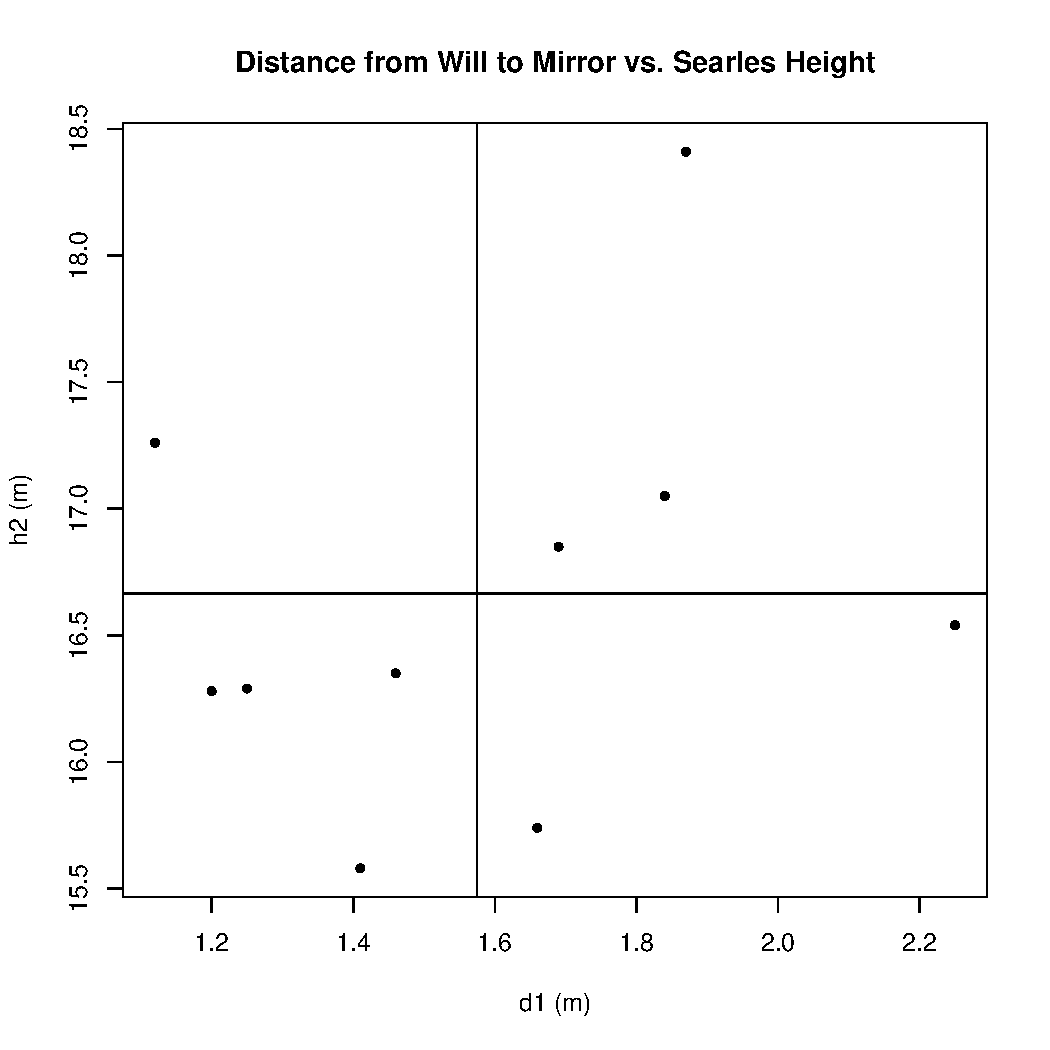
\includepdf[scale=0.8]{d1_h2.pdf}
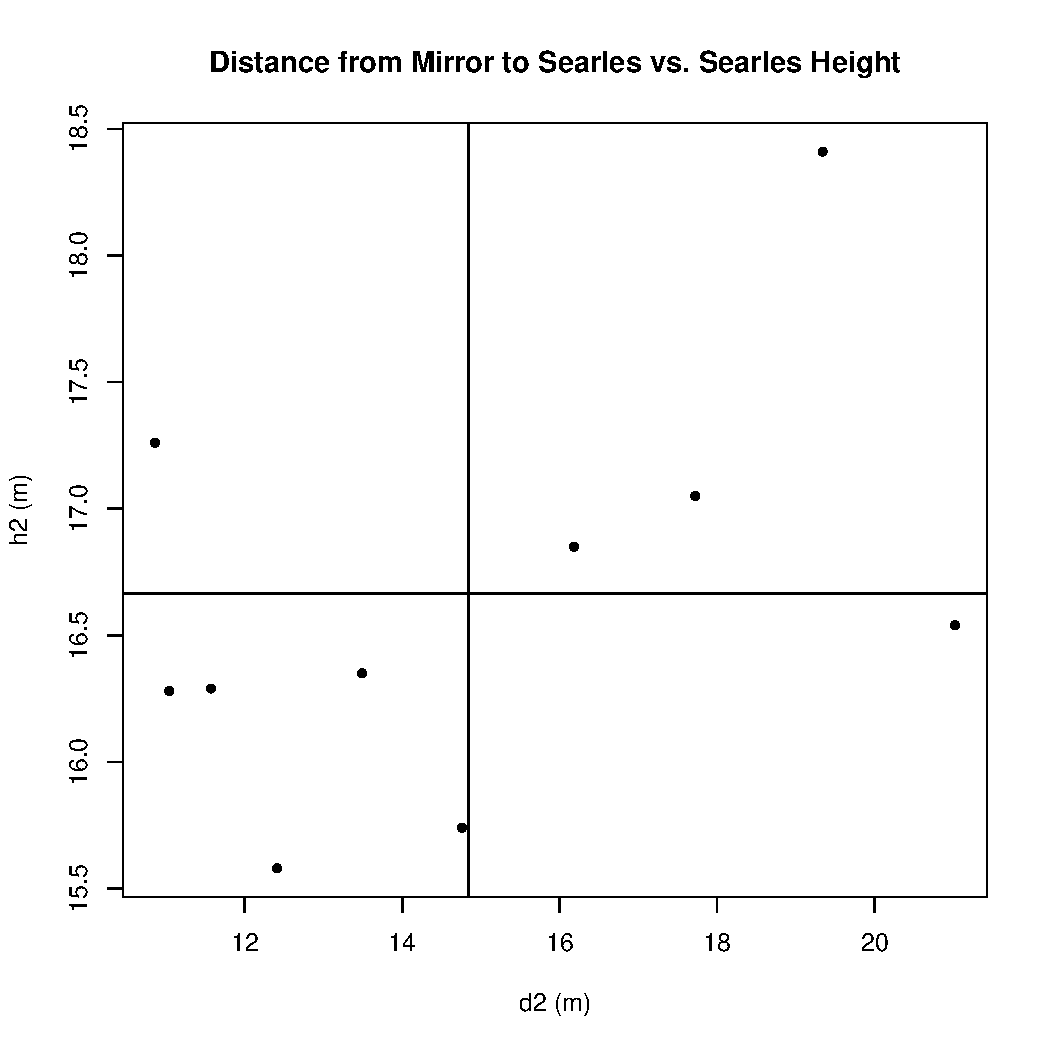
\includepdf[scale=0.8]{d2_h2.pdf}
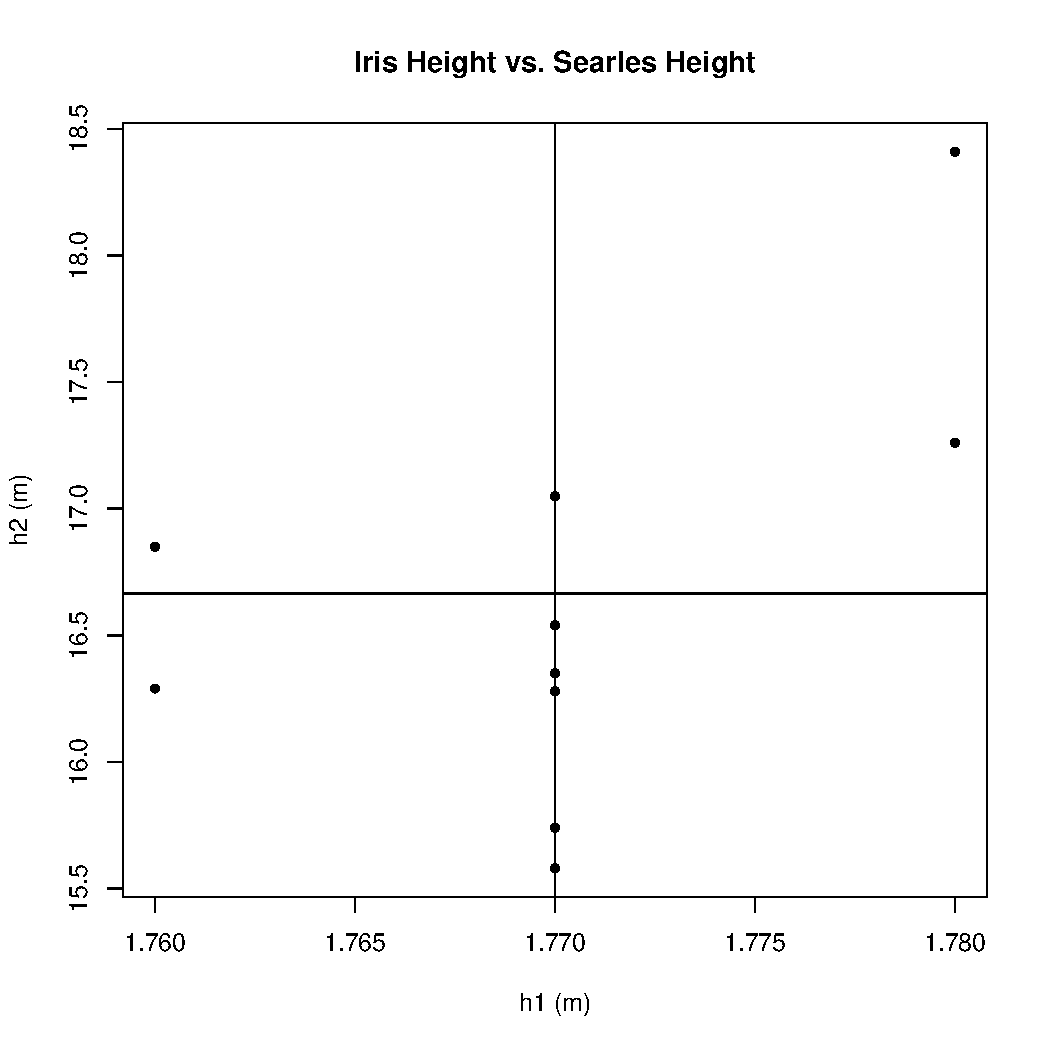
\includepdf[scale=0.8]{h1_h2.pdf}

\end{document}